\section{การนำเสนอภาพ}

\hspace{1cm} ก่อนจะนำเสนอขั้นตอนวิธีเชิงตัวเลขชนิดใหม่จะขอกล่าวถึงการนำเสนอภาพเชิงคณิตศาสตร์ ดังนี้

\subsection{การนำเสนอภาพเฉดเทา}

\hspace{1cm} กำหนดให้ $I : \Omega \subset \mathbb{R}^2 \rightarrow V \subset [0,\infty)$ แทนภาพเฉดเทา (grayscale image)  เป็นฟังก์ชันต่อเนื่อง โดยที่ $ \mathbf{x} = (x,y) \in \Omega $ แทนพิกัดทางกายภาพ (physical position) ของภาพ $ I(\mathbf{x}) \in V $ แทนระดับความเข้มของภาพ (image intensity) ที่ $ \mathbf{x} $ และ $ \Omega $ แทนโดเมนของภาพซึ่งเป็นรูปร่างสี่เหลี่ยม ซึ่งในที่นี้สามารถสมมติได้โดยไม่เสียหลักการสำคัญว่า $ \Omega = [1,n]^2 $ และ $ V = [0,1] $ เมื่อ $n>1$ เป็นจำนวนเต็มบวก 

\begin{figure}[H]
    \centering
    \begin{subfigure}{0.8\linewidth}
        \centering
        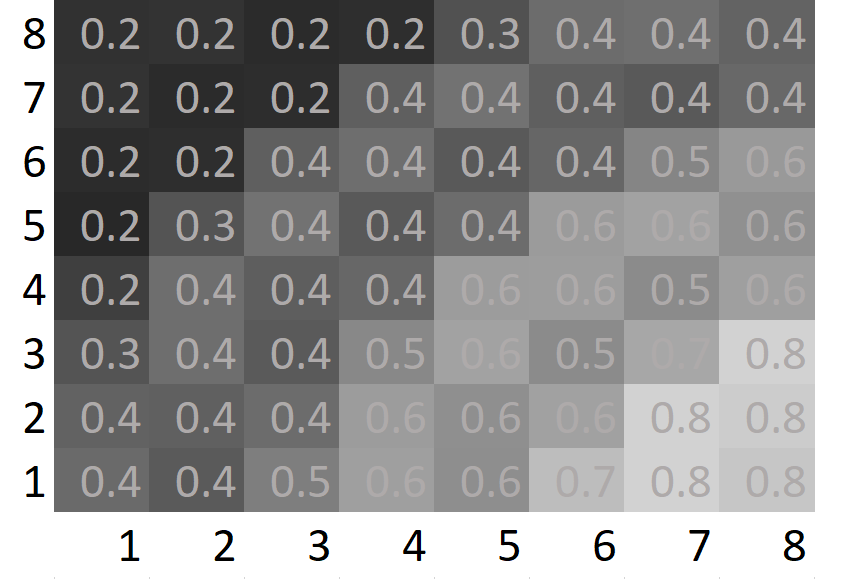
\includegraphics[width=0.45\linewidth]{image/grayscale-explain.png}
    \end{subfigure}
    \caption{ตัวอย่างภาพเฉดเทาที่แสดงระดับความเข้มของภาพในแต่ละระดับ}
    \label{figure:grayscale-explain}
\end{figure}

\hspace{1cm} จากภาพ \ref{figure:grayscale-explain} สังเกตว่าที่ค่าความเข้มของภาพเข้าใกล้ 0 จะให้สีเป็นลักษณะสีดำ ดังเช่นบริเวณที่พิกัดทางกายภาพเป็น (4,8) และเมื่อค่าความเข้มของสีเข้าใกล้ 1 จะให้สีที่มีลักษณะเป็นสีขาว ดังเช่นบริเวณที่มีพิกัดทางกายภาพเป็น (7,1)

\subsection{การนำเสนอภาพสี}

\hspace{1cm} กำหนดให้ $ \boldsymbol{I} = (I_1,I_2,I_3)^{\top} : \Omega  \rightarrow V^3 $ แทนภาพสีในระบบ RGB เมื่อ $I_1,I_2,I_3: \Omega  \rightarrow V$ แทนส่วนประกอบสีแดง สีเขียว และสีน้ำเงินตามลำดับ

